\chapter{Personal Experience}

From interview to the end of my internship and beyond, I passed a great time at Kaz Software.
In this chapter, I'll go through those experiences.

\section{Interview}

I had a phone interview with Shawal Siddique (CTO, Kaz Software).
It was not a formal interview.
He called and asked me questions about in what technology I worked on, questions about ReactJS, how I like my work environment etc.
He confirmed my internship in that call.

\section{Team Artisan}

As an intern, I joined the Team Artisan in Kaz Software.
It is a team with some talented and friendly members.
I worked for six months as an intern in that team, and joined as an Associate Software Engineer later.

\subsection{Members}

Team Artisan consists of some great members, who are talented, friendly and helpful at the same time.
Currently there are nine members, including me, in Team Artisan.

\begin{itemize}
    \item Md. Hannan Hossain (Team Lead, Principal Software Engineer)
    \item Mohammed Jubayer (Principal Software Engineer)
    \item Biswajit Panday (Senior Software Engineer)
    \item Tulshi Das (Software Engineer)
    \item Ashiqur Rahman Rijvy (Associate Software Engineer)
    \item Saikat Sen (Associate Software Engineer)
    \item Souhardya Saha (Associate Software Engineer)
    \item Siana Rizwan (Intern) 
\end{itemize}

Four more ex-members of the team I must mention are:

\begin{itemize}
    \item MD. Ibrahim Khan (currently working as a software engineer at Cefalo Bangladesh Ltd.)
    \item Md Masum (changed team)
    \item Abdullah-Al Foysal (changed team)
    \item Abdullah Al Jahid (internship period is over)
\end{itemize}

\begin{figure}[h]
    \begin{center}
        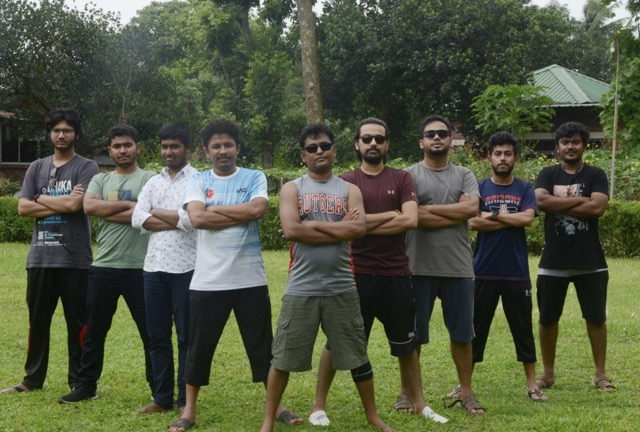
\includegraphics[width=0.9\textwidth]{images/Chapter3/artisan.jpeg}
        \label{fig:team_artisan}
    \end{center}
\end{figure}

\subsection{Office Hours}

Kaz has different office hours for different teams.
Team can choose office hours according to their ease.
But each team should work for 8 hours, 5 days a week with one hour of lunch break at 2:00 PM.
Team Artisan starts working at 11:00 AM and ends at 7:00 PM.

\subsection{Scrum}

Each working day at 11:00 AM, all of the members of Team Artisan have a scrum meeting.
Every member must join the meeting unless they are on leave.
In this scrum meeting members discuss:

\begin{itemize}
    \item What did they do the last day
    \item What will they work on today
    \item Issues and blockers they are facing
\end{itemize}

\subsection{CTO Meeting}

On Tuesday 3:00 PM of every first full week of a month the members of Team Artisan have a meeting with the CTO.
In this meeting they discuss about the progress of the projects the team currently working on, the wellbeing of the member and the members' real life events.
Every member of the team must join this meeting.

\subsection{Fine Driven Development}

FDD is a fun terminology, but it is strictly followed in Team Artisan.
There is a fine if a member misses the scrum meeting or CTO meeting.
There is fine for committing code with silly mistake or deploy a buggy code to the production.
And there is a rule book for the team, and if a member break any rule, s/he might get a fine.
There is also a fee for a Kazian when s/he joins or leave the team.
The fine amount is small and the fund created from these fines are used for recreation of the team, like a party or a tour.

\section{Pair Programming and Collaboration}

Pair programming is an agile software development technique in which two programmers work together at one workstation. One, the driver, types in code
while the other, the observer (or navigator), reviews each line of code as it is typed in. The two programmers switch roles frequently.\\

From the second day of my internship I started pair programming with MD. Ibrahim Khan bhai and Md Masum bhai.
As I was new to the Orbitax ecosystem, I always had a lot of questions.
Therefore, I could clear my confusion while talking with the seniors and gain knowledge about the platform.
And later when Abdullah Al Jahid and Siana Rizwan joined Team Artisan, we started pair programming as we worked on the same project.\\

While working as a pair, we used to work in a way, when my partner was typing I was assisting him, giving him ideas and checking for mistakes; when I was typing my partner was giving me instructions.
It is easier to find bugs and corner cases during development and write efficient code when two or more people write code together.\\

The best thing about Kaz Software is, people here never hesitates to ask for help.
Whenever I got stuck, could not understand a legacy code or had trouble understanding what to do, I asked for help from my seniors.
No matter whatever the problem was, they always helped me and this made my internship period a lot smoother.\\

I tried to help others too.
As for using ReactJS for a long time for web development, I was able to help my fellow interns and even my seniors who had confusion about ReactJS.
Although every team of Kaz Software works separately, anyone can ask for help from anyone from any team.

\section{Recreation} 

Kazians always works in a fun way.
The recreations in Kaz Software are already discussed in the Company Profile section.
I was lucky that I could join almost every tour, outing, and party even when I was an intern.

\section{Remuneration}

Although this internship was a part of our undergraduate curriculum, I was given a salary of a good amount.
I am not allowed to share the exact number of my salary but it was enough to cover my basic needs as a student.
Later they offered me a full time job, with more than 250\% of the monthly salary I used to receive during internship.

\section{Full Time Job}

After completing my internship I had a long free time before my university class started.
So, Wahid Choudhury Bhai and Shawal Siddique bhai proposed me an offer to join as an Associate Software Engineer at Kaz Software.
I accepted the offer without any hesitation as he offered me flexibility to take leave when my university classes start.
I was happy to join the team I completed my internship in.
